\section{State of the art in ESD testing}

To ensure proper operation once in the field, hardware is tested against \gls{esd} using different test methods and standards.
The goal for each method is to reproduce a particular \gls{esd} waveform in lab conditions.
In this chapter, we will introduce most relevant \gls{esd} generators, which will be useful later on for modeling them accurately.

In ESD testing, distinction is often made between so-called system-level level tests and \gls{ic} level tests.
The first kind reproduces \gls{esd} events that a system deployed in the field may encounter during its lifetime, while the latter is targeting \gls{esd} events
happening during \gls{ic} manufactoring.

System-level tests involve higher voltage and current amplitudes, and are more harmful for electronic devices than \gls{ic} level tests.
EXTERNAL DEVICES FOR PROTECTING ?
ICs now have to sustain SYSTEM level tests

\subsection{Transmission Line Pulsing (TLP)}

\gls{tlp} generators generate a fast rectangular pulse \ref{tlp_concept}.
The pulse is produced by the discharge of a coaxial cable.
The cable is charged by a high-voltage power supply then discharged into a load by switching a relay.

\begin{figure}[h]
  \centering
  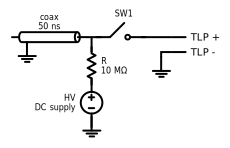
\includegraphics{src/1/figures/tlp_concept.pdf}
  \caption{Minimal example of a \gls{tlp} system}
  \label{tlp_concept}
\end{figure}

The charge is performed through a high value resistor to keep the current small and avoid generating oscillations on the cable.

TLP systems constitute very well-controlled test generators, because the pulse is generated inside a shielded and isolated environment.
Characteristic impedance can be controlled up to the load.
Those features allow for extremely clean and repeatable pulse waveforms.
Main characteristics of a TLP waveform are given in figure \ref{tlp_pulse}

\begin{figure}[h]
  \centering
  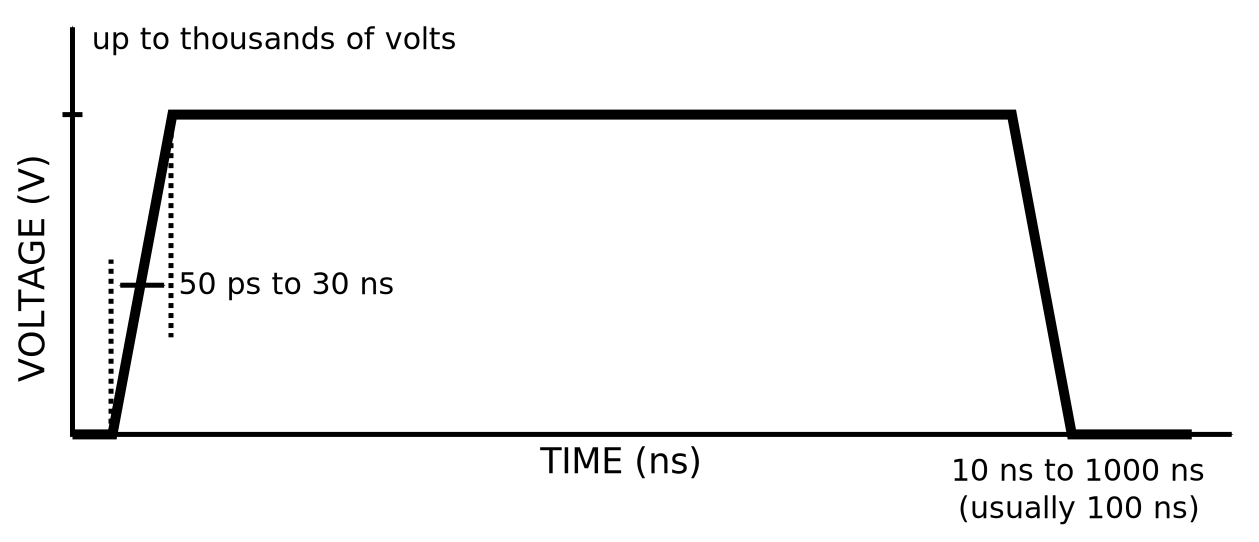
\includegraphics[width=\textwidth]{src/1/figures/tlp_pulse.pdf}
  \caption{Main characteristics of a \gls{tlp} pulse on a resistive load}
  \label{tlp_pulse}
\end{figure}

Using time-domain reflectometry, it is possible to reconstitute the current and voltage waveforms inside the load,
from measured current and voltage inside the \gls{tlp} \cite{TLP}.
The superposition of the incident and reflected pulses during the discharge show that the voltage and current
measured inside the generator are direct image of the ones accross and through the load.

\gls{tlp} are extensively used for characterizing the response of ESD protections \cite{TLPforESDProtectionCz}
or testing the response of systems and devices against a clean and well repeatable pulse \cite{TLPthroubleshooting, LacrampeTransientImmunity}.

\subsection{ESD Gun (IEC 61000-4-2 / ISO 10605)}
The system-level ESD Gun aims at reproducing the discharge of a human body through an electronic device.
This test is used extensively for the qualification of products.

\begin{figure}[h]
  \centering
  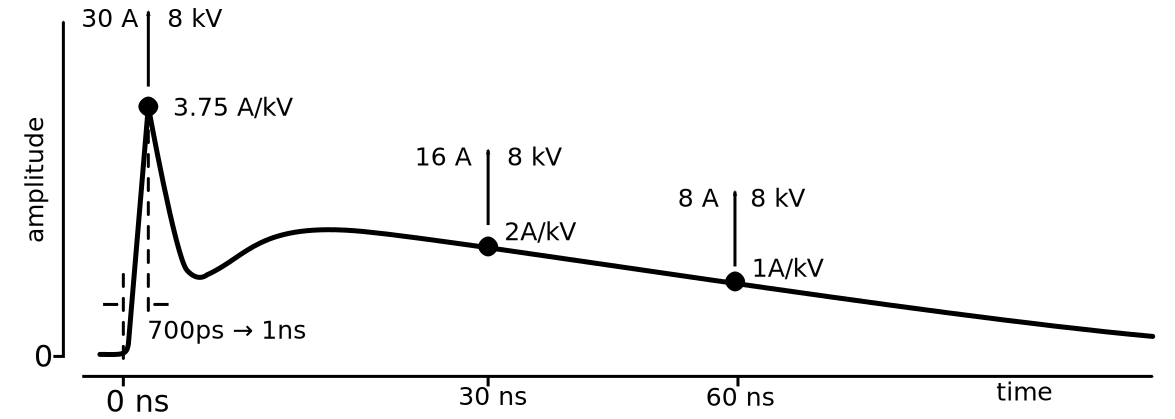
\includegraphics[width=\textwidth]{src/1/figures/iec61000-4-2_waveform.pdf}
  \caption{Main characteristics of an IEC 61000-4-2 pulse on a 2&\X\Omega resistive load}
  \label{iec_pulse}
\end{figure}

The generation of the ESD pulse is done by an resistor-capacitor discharge network, however, the RC network alone does not suffice to reproduce the waveform given \ref{iec_pulse}.
Parasitic devices play an important part in shaping the waveform.

Two standards define the construction and waveform requirements for this ESD generator, but with different fields of application.

IEC 61000-4-2\cite{iec61000-4-2} standard targets consumer electronics, while ISO 10605\cite{iso10605} standard is intented for automotive equipment.
The latter defines additional pulse waveforms to cover a wider range of ESD events (See fig \ref{iso_pulse}).

\begin{figure}[h]
  \centering
  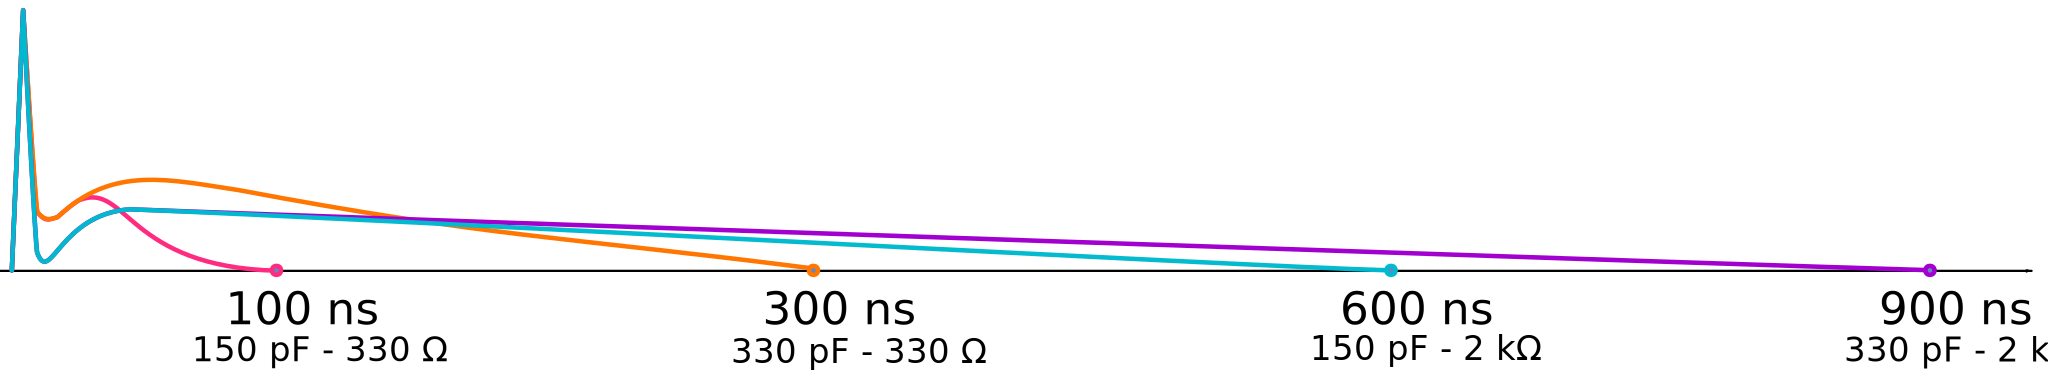
\includegraphics[width=\textwidth]{src/1/figures/iso10605_waveform.pdf}
  \caption{All waveforms defined in ISO 10605 standard on a 2&\X\Omega resistive load}
  \label{iso_pulse}
\end{figure}


\subsection{ISO 7637-2}
ISO 7637-2\cite{iso7637-2} is an automotive standard for testing immunity of electronic devices against transient electrical disturbances.
It is mostly targeting disturbances applied on supply lines.
This standard gathers many different pulses. Pulse 2A and 3B are in the ESD timescale.

Pulse 2A simulates the sudden disconnection of a load placed in parallel with the \ref{dut}.

SCHEMA

The parasitic inductance of the wiring harness is opposing to this interruption of current.
Instead of flowing through the load, this extra transient current is reported on the \ref{dut} which can be damaged or disturbed in the process.

The characteristics of pulse 2A are given in fig. \ref{...?}

PULSE 2A waveform

On the other side, pulse 3B simulates the result of a switching process with a wiring harness.
The waveform is similar to pulse 2a, but with a shorter duration and risetime and higher amplitude.

PULSE 3A waveform

\subsection{Burst test (IEC 61000-4-4)}

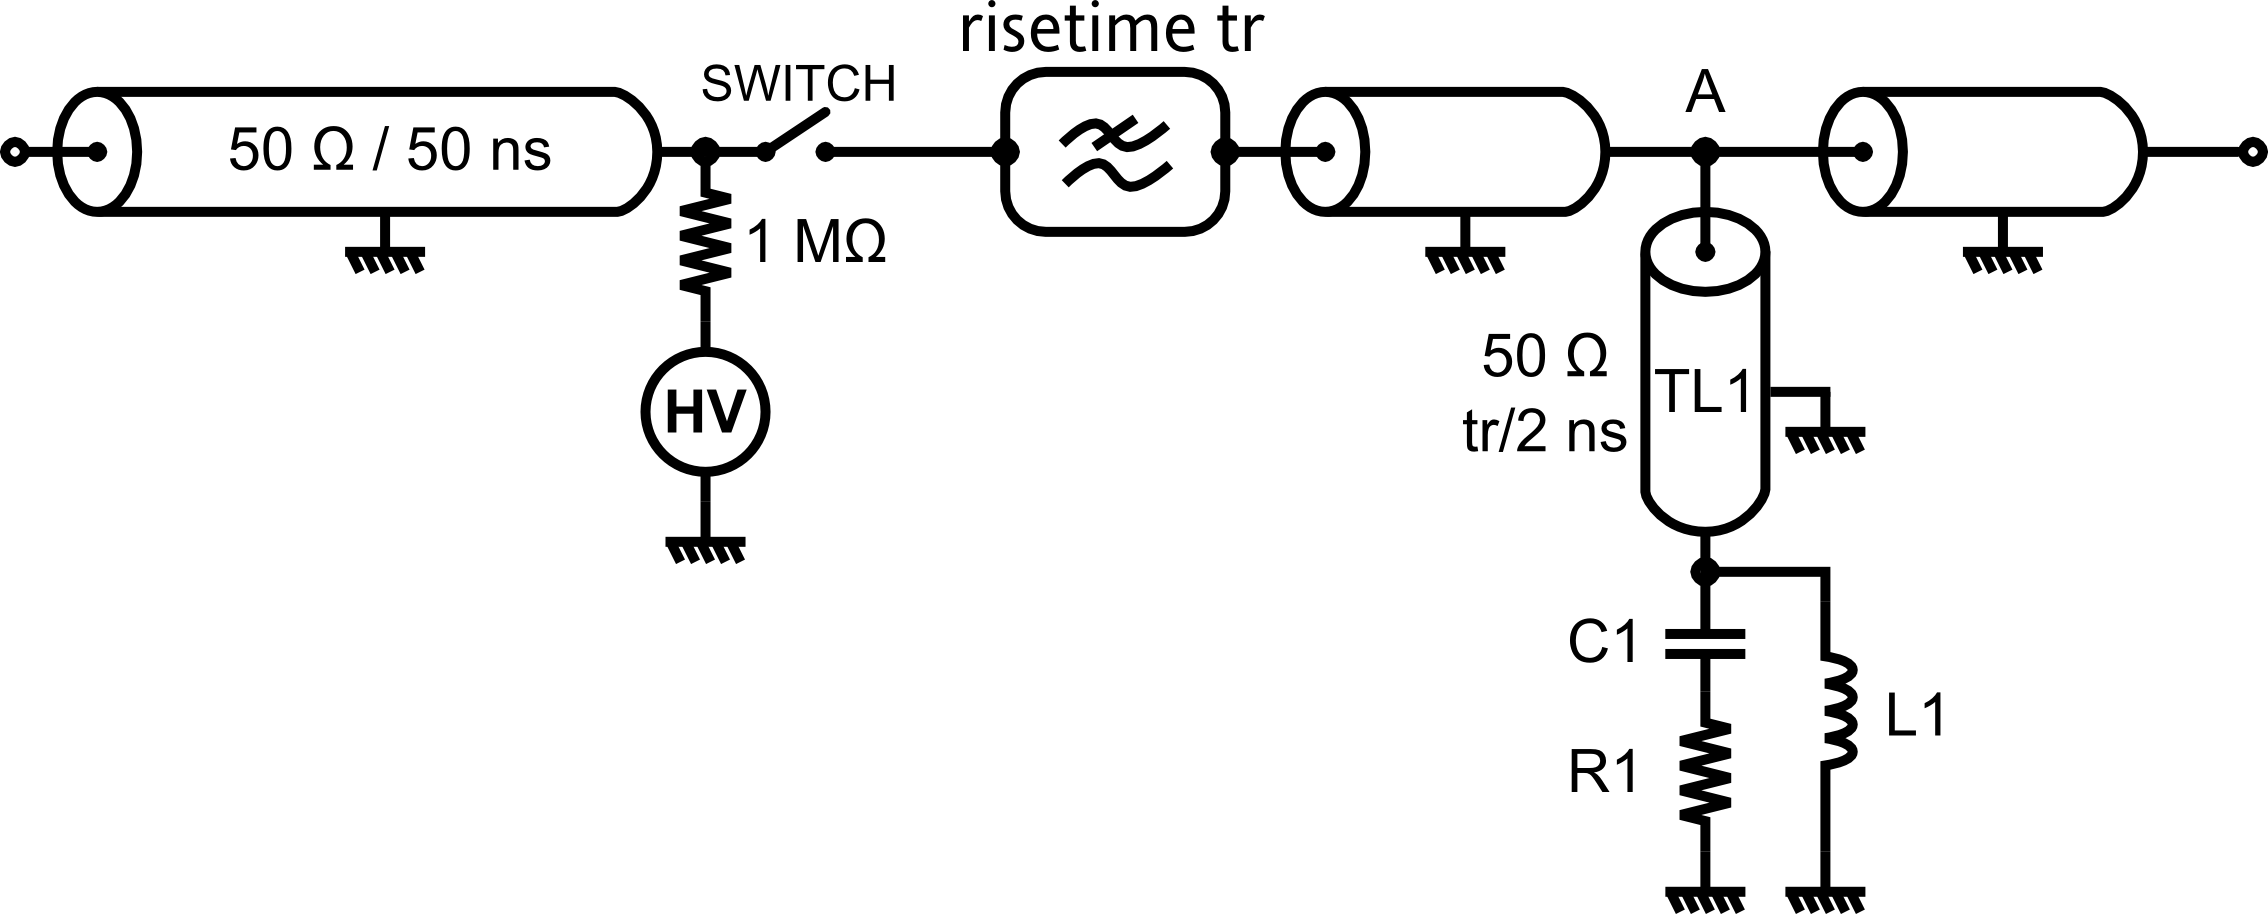
\includegraphics[width=\textwidth,height=\textheight,keepaspectratio]{src/2/figures/tlp_iec.png}
